\section{Explanations on PCA model order reduction}

%Some words on PCA, learn of 2 Matrix full-dim to reduced-dim and back.
%Then how we use it (pictures and text).

Figure~\ref{fig.MNIST} illustrates the pipeline used for MNIST benchmark. The MNIST dataset was used to directly train a MNIST DNN, achieving 97\% accuracy, as denoted by ``Training''. 
%
It was also used to obtain the PCA encoding and decoding, transforming the images into a reduced basis. The number of PCA dimensions was chosen such that the exploitation accuracy remains constant. That is, encoding into a PCA basis and decoding it results in the same accuracy, as illustrated in ``Exploitation''. 
%
Last, for the ``bound computation'', we determine an $L_1$-perturbation $\varepsilon$. The search space for bound computation is 20-dimensional. However, the bound itself is computed on the full-space. This is possible since PCA is a \emph{linear operation} based on the eigenvectors of the covariance matrix and its transpose for the PCA decoding (inverse).

\begin{figure*}[]
	\centering
	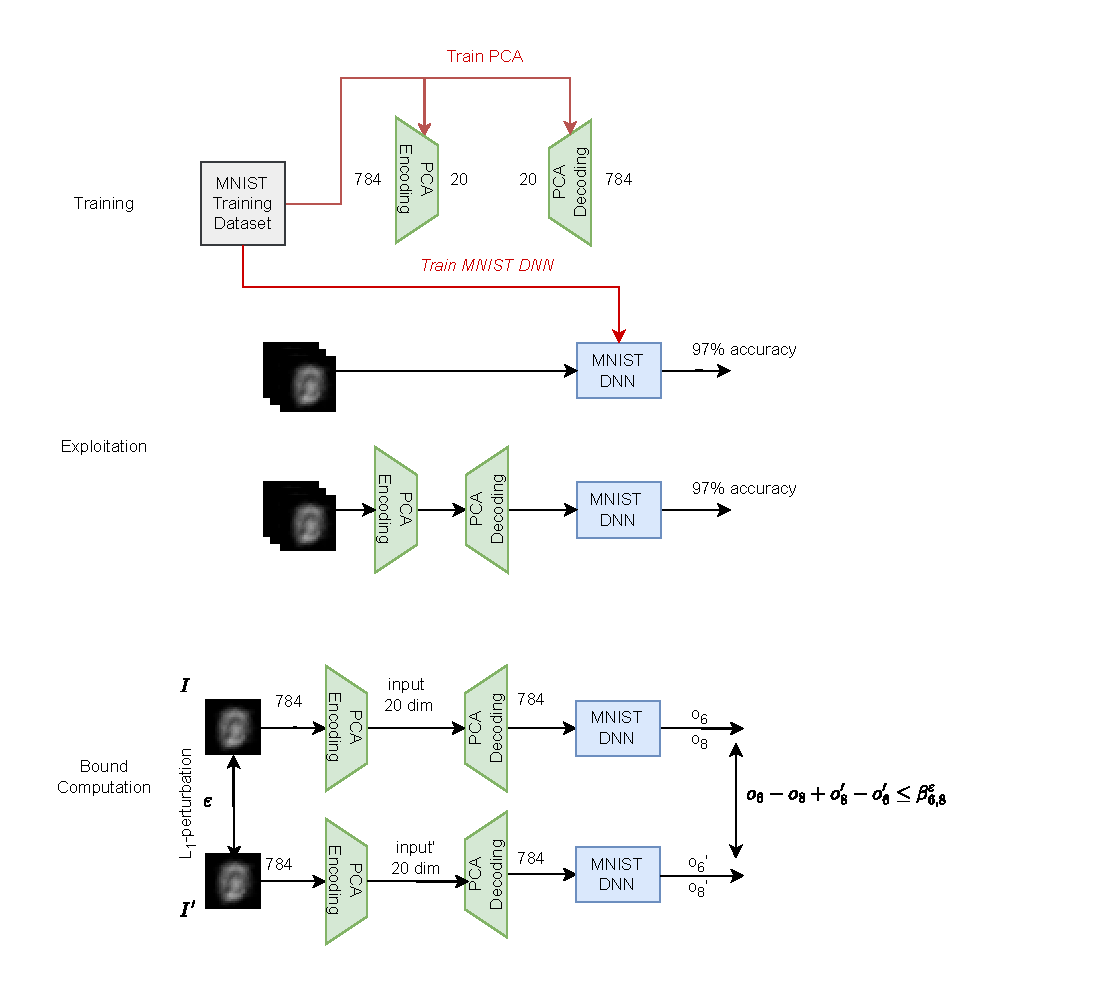
\includegraphics[scale=0.9]{MNIST.pdf} \hspace{1.5cm}
	\caption{Training, exploitation and bound computation on the MNIST dataset. Note that PCA encoding/decoding used back-to-back allow to maintain the same accuracy. In addition, the bound is computed on the full-space even though the analysis is performed on the reduced space. dim = dimension.}
	\label{fig.MNIST}
\end{figure*}	

Figure~\ref{fig.PIPE} illustrates the same pipeline used in the pipe strain case. In this case, two different PCA are used. The first one is learned with the deformation training dataset and the second is learned with the plastic strain one. 
%
The surrogate is then learned from the reduced deformation to the reduced plastic strain. 
%
For exploitation, we obtain the deformation, use the PCA basis to obtain a reduced deformation, fed the reduced deformation to the surrogate obtaining the reduced strain and decode the strain (apply PCA inverse), obtaining the strain in the full pipe geometry. Similarly to the MNIST case, we obtain a bound $\varepsilon$ on the input space by solving the MILP problem as proposed on the input dimension.

\begin{figure*}[]
	\centering
	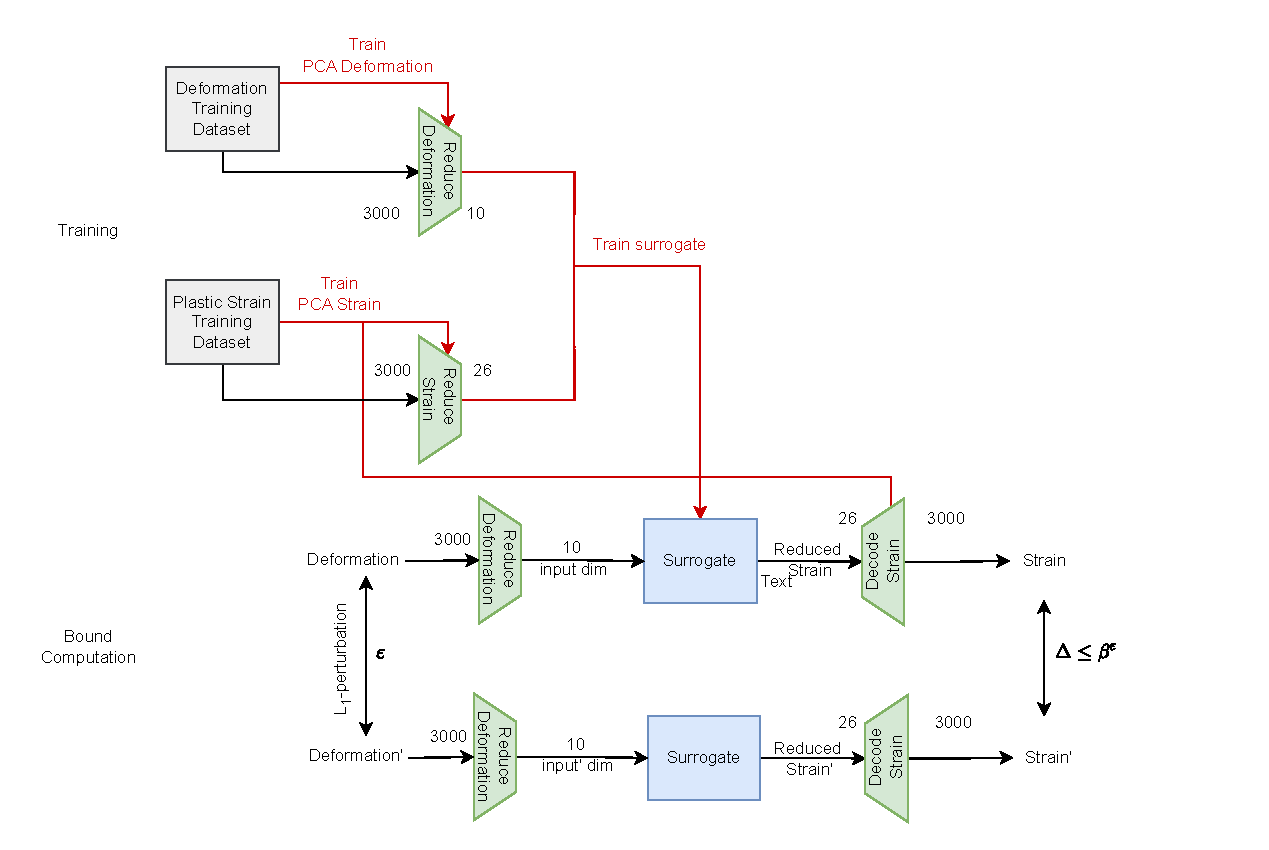
\includegraphics[scale=0.9]{PIPE.pdf} \hspace{1.5cm}
	\caption{Training and bound computation on the pipe use case. Note that two PCA are used, one for the input space (deformation) and another for the output space (plastic strain). The exploitation and bound computation must then use a pipeline that: (1) reduces the deformation; (2) obtain a reduced strain with the surrogate and (3) decodes the reduced strain using the PCA inverse. dim = dimension.}
	\label{fig.PIPE}
\end{figure*}	
